\documentclass[../main.text]{report}
\subsection{Ressemblence et differences entre ensembles aléatoires et nombres premiers}

Nous voulons maintenant comparer les groupes entre eux. Pour cela, nous allons mesurer, pour chaque ensemble, le rapport $\frac{\sigma_k(n)}{\pi(n)}$ où $\sigma_k(n)$.

\begin{figure}[H]
	\centering
	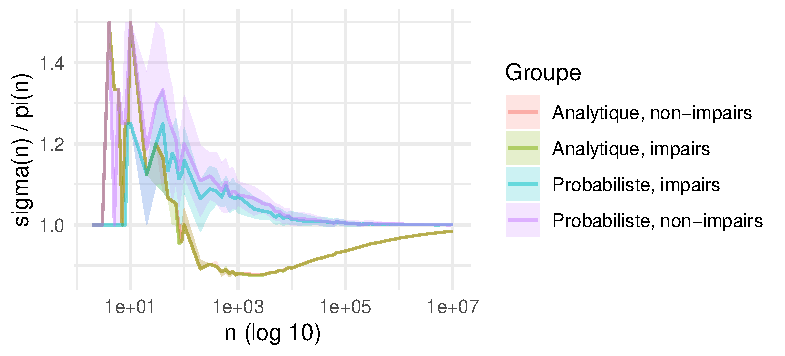
\includegraphics{comparison_all_random_sets}
	\caption{Rapport entre $\sigma(x)$ et $\pi(x)$. La courbe représente la médiane et la surface autour de la courbe les premier et troisième quartiles. }
	\label{fig:comparison_all_random_sets}
\end{figure}


Nous savons maintenant que les ensembles aléatoires suivent assez fidèlement $\pi(x)$. Nous souhaitons alors mesurer à quel point ces ensembles sont différents. Soit $R_n$ l'ensemble dont nous souhaitons mesurer la ressemblance à $P_n := \{p~\in~\mathbb{N}~|~p$~est~premier, p < n$\}$ . Nous calculons alors le cardinal de $R_n \cap P_n$ puis divisons ce nombre par le cardinal de $R_n$ afin d'obtenir, en pourcentage, la proportion d'élements premiers de $R_n$.

La figure \ref{fig:intersection_primes} montre cette proportion pour chaque groupe d'ensemble. 

\begin{figure}[H]
	\centering
	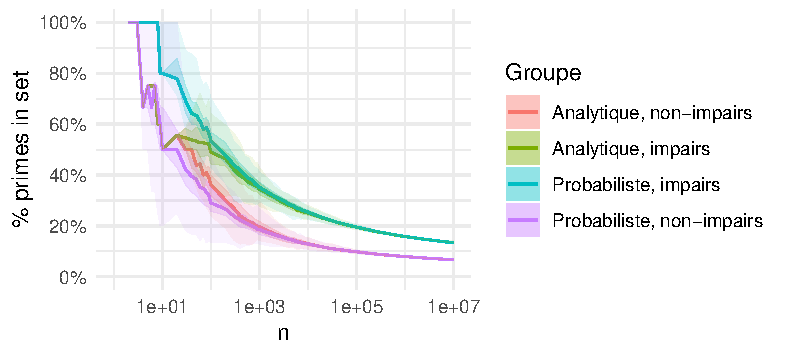
\includegraphics{intersection_primes}
	\caption{Proportion de nombres premiers dans les ensembles aléatoires en fonction de $n$, en pourcentage. La courbe représente la médiane, la surface autour de la courbe les premiers et troisièmes quartiles.}
	\label{fig:intersection_primes}
\end{figure}

À partir de $10^3$, moins de la moitié des élements des ensembles sont des nombres premiers. 
Dès $10^5$,  les nombres premiers ne représentent plus que 10\% des ensembles impairs, et 20\% des ensembles non-impairs. 
De plus, il n'y a pas de différence significative entre deux ensembles d'un même groupe dès lors que $n$ est assez grand. 